\href{https://github.com/JuliaReach/LazySets.jl}{LazySets.jl} is an open-source Julia package for calculus with geometric sets of points in Euclidean space (for a visual example see Fig.~\ref{fig:lotka_volterra}).
That is, the package provides solutions to represent sets, perform calculations on them, and combine them via set operations to form new sets.
A key aspect of LazySets is that set operations can be applied concretely, meaning that a computation is invoked, or lazily, meaning that the computation is delayed.
Crucially, based on geometric concepts, LazySets can evaluate queries on the lazy set representation, which enables efficient operation in very high dimensions that is not possible when applying the operations concretely.

\smallskip

LazySets aims to be a flexible and scalable library.
%
It provides specialized representations for various common classes of sets and ways for interacting with these sets, and is able to work with complex set constructs by use of the support-function calculus.\footnote{Complementary background is included in the Appendix.}
%
Flexibility is achieved by implementing generic algorithms that apply to multiple types of sets, and interoperability is achieved by connecting all set types through common interfaces.
%
Efficiency is achieved by adding special-case implementations where applicable; set operations are often binary functions and Julia's multiple dispatch greatly simplifies the choice of the most efficient implementation for a given combination of sets.
%
LazySets is designed to work with very high-dimensional sets but also provides specialized methods for one- and two-dimensional sets.
%
Finally, LazySets is well integrated with the Julia ecosystem for scientific computing~\cite{bezanson2017julia}, and additional functionality is available upon loading optional packages.
%

\smallskip

In this article we present the basic functionality of LazySets, starting with common sets and operations in Section~\ref{sec:basic}.
%
More advanced topics on type composition and conversion are introduced in sections \ref{sec:lazy} and \ref{sec:approx}.
%
Several applications are included in Section~\ref{sec:applications}.
%
We provide references and comment on related libraries in Section~\ref{sec:conclusion}.
%
Installation instructions can be found in Appendix~\ref{sec:installation}.
%
Background mathematical definitions are included in Appendix~\ref{sec:mathdef}.
%
The code to reproduce the figures can be found in Appendix~\ref{sec:code_examples}.

\begin{figure}[t]
	\centering
	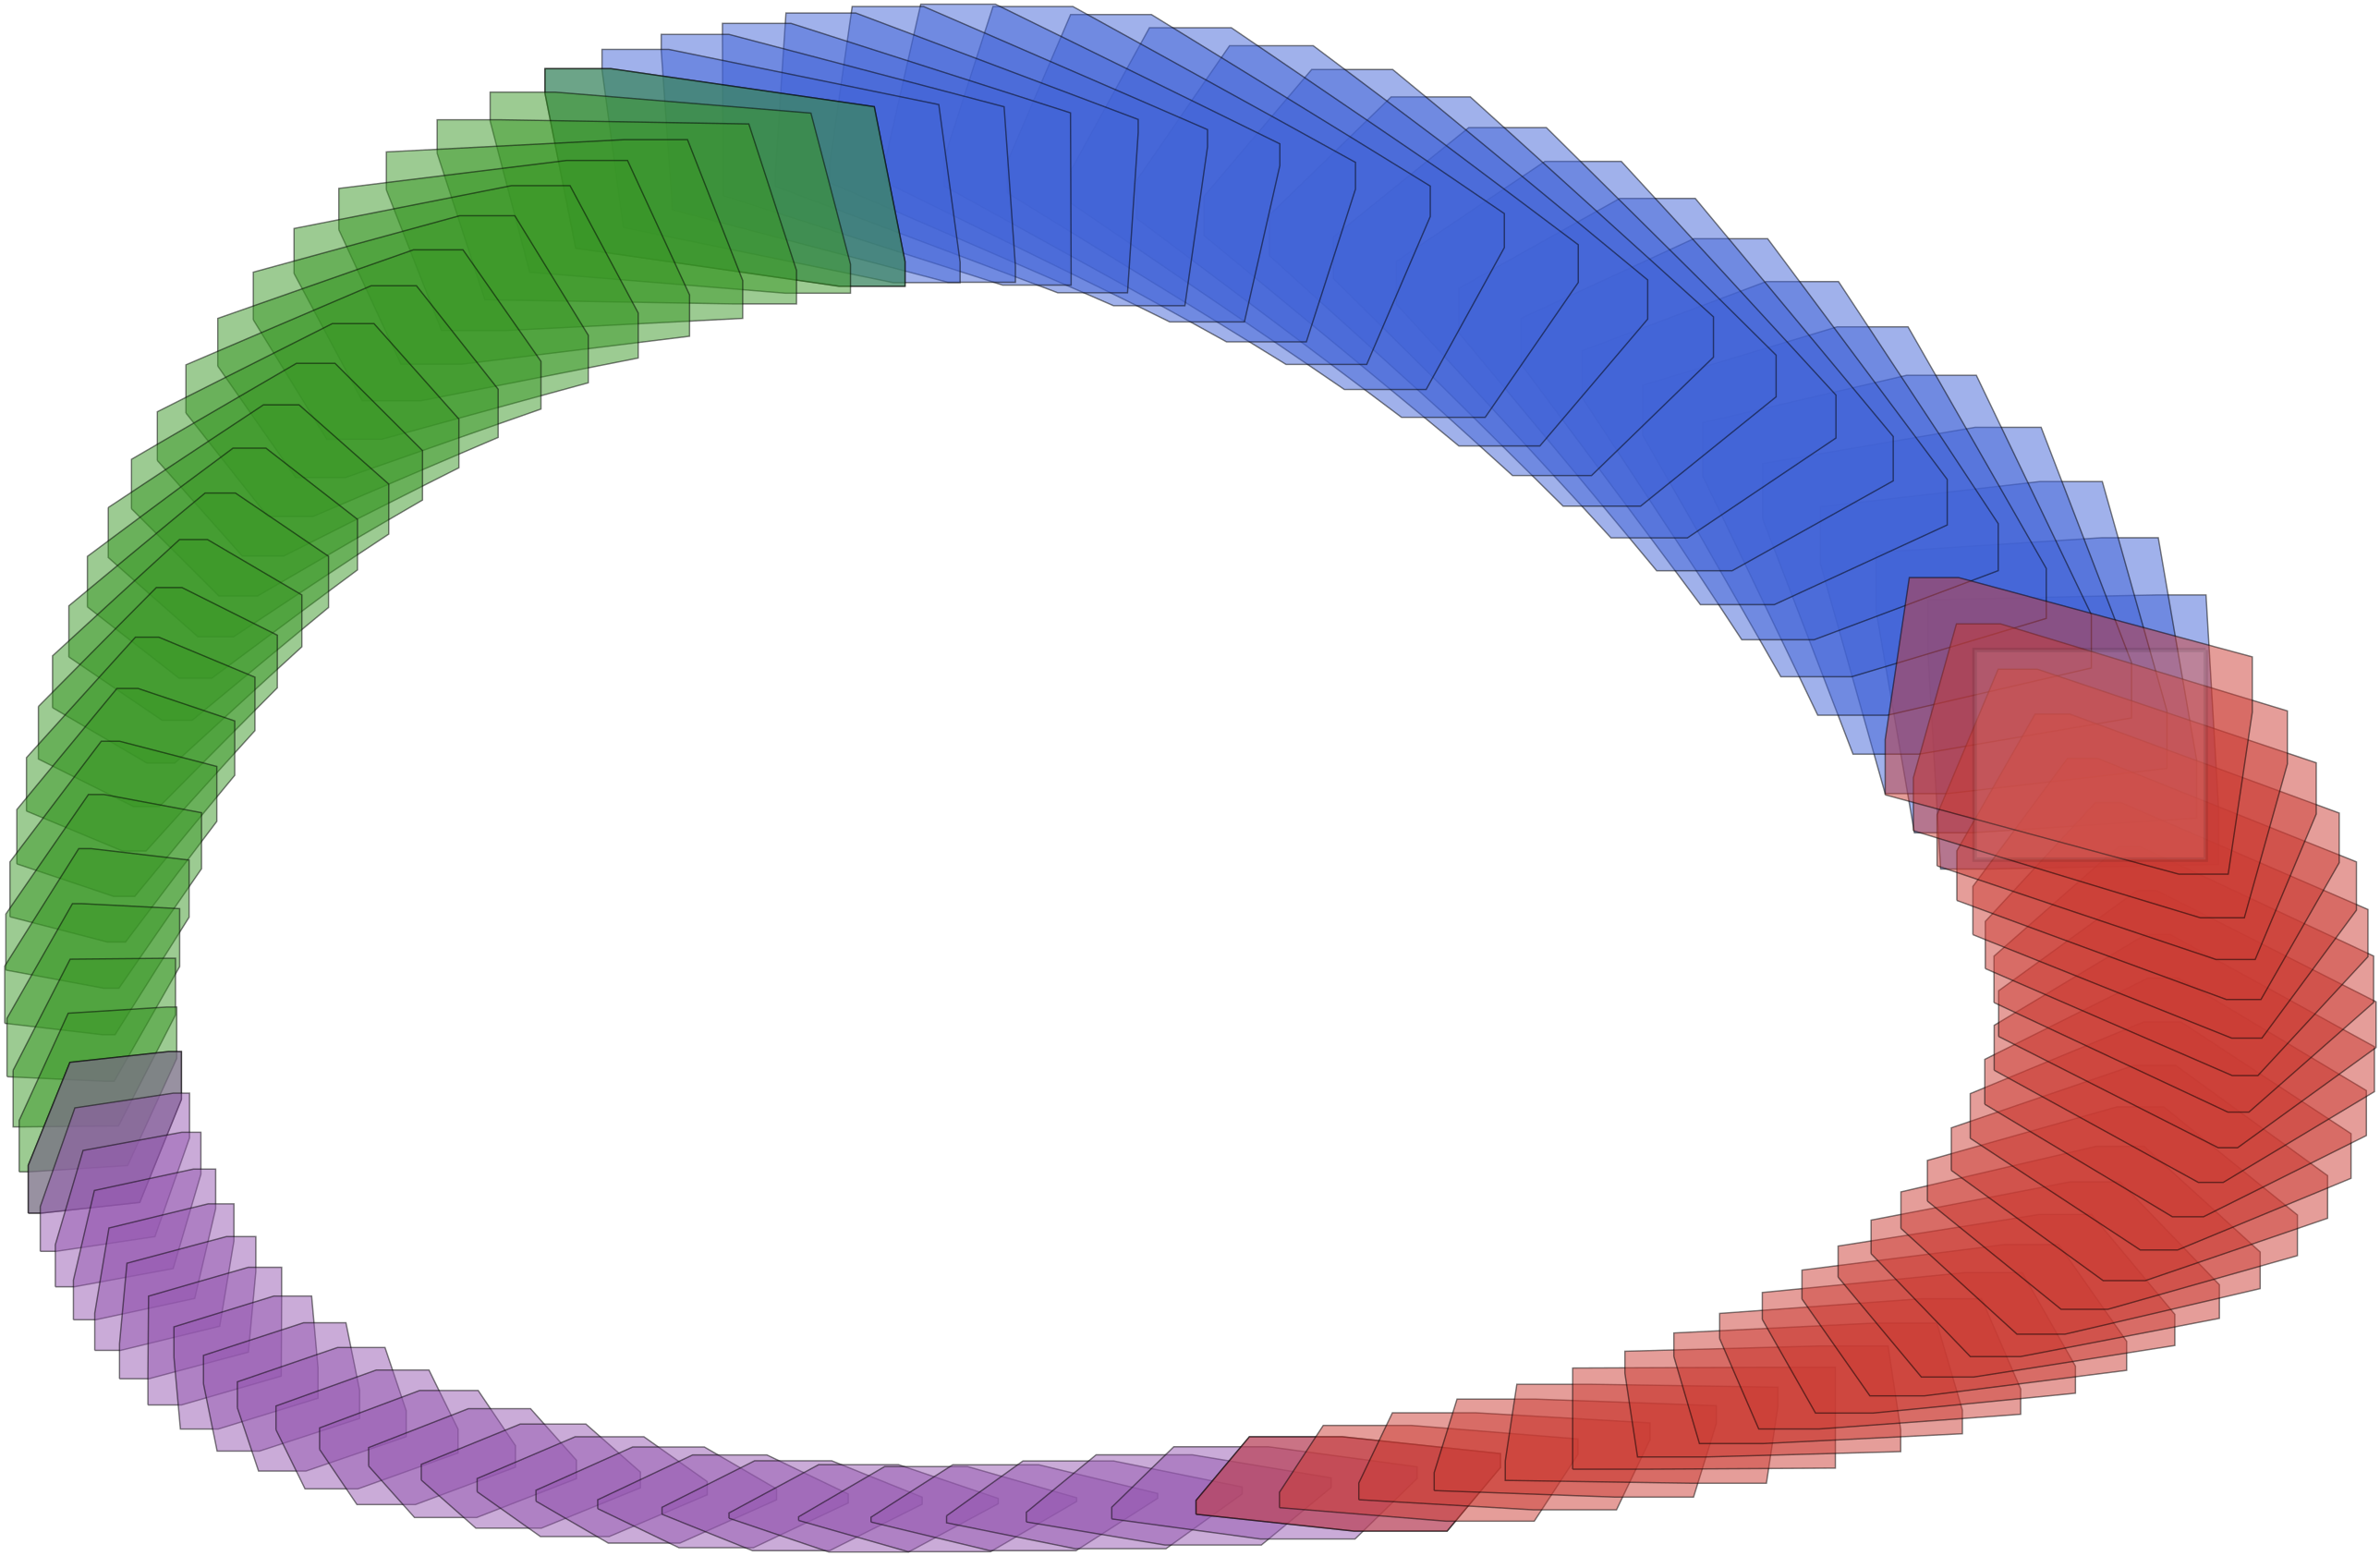
\includegraphics[width=0.7\linewidth, keepaspectratio]{img/lotkavolterra}
	\vspace*{1mm}
	\caption{Example of set propagation using LazySets.}
	\label{fig:lotka_volterra}
\end{figure}
